% Tento soubor nahraďte vlastním souborem s přílohami (nadpisy níže jsou pouze pro příklad)
% This file should be replaced with your file with an appendices (headings below are examples only)

% Umístění obsahu paměťového média do příloh je vhodné konzultovat s vedoucím
% Placing of table of contents of the memory media here should be consulted with a supervisor
%\chapter{Obsah přiloženého paměťového média}

%\chapter{Manuál}

%\chapter{Konfigurační soubor} % Configuration file

%\chapter{RelaxNG Schéma konfiguračního souboru} % Scheme of RelaxNG configuration file

%\chapter{Plakát} % poster

\chapter{Screenshots}

\begin{figure}
	\begin{center}
		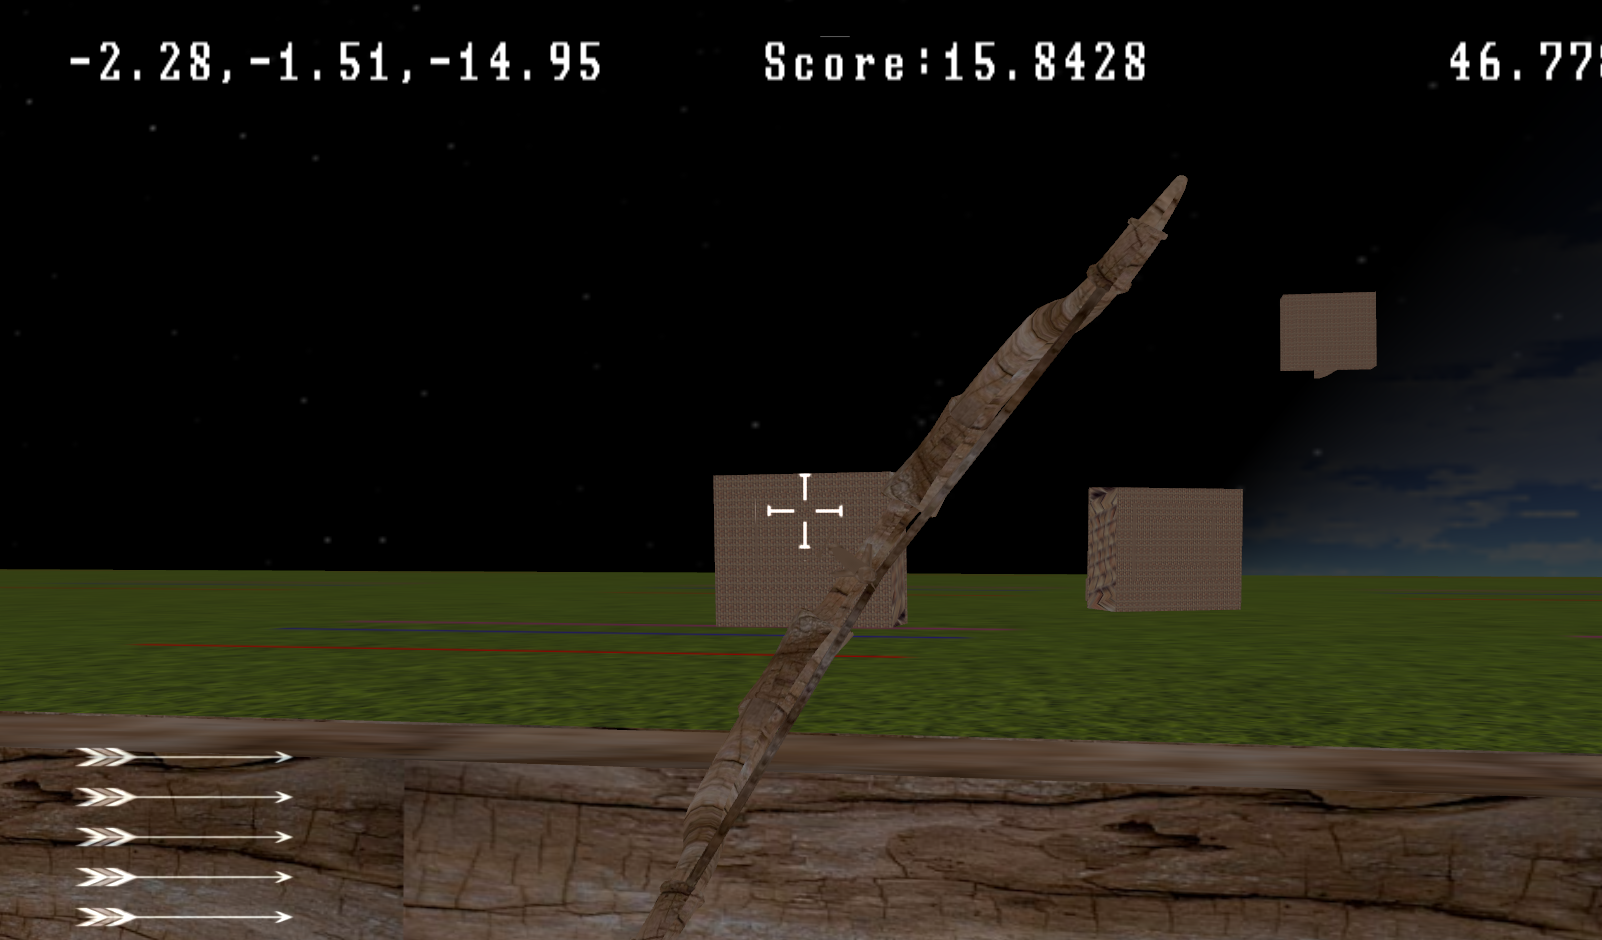
\includegraphics[scale=0.25]{obrazky-figures/22}
		
		\caption{Screenshot ze střelecké pozice s naplým lukem}\label{screenShot1}
\end{center}\end{figure}
\begin{figure}
	\begin{center}
			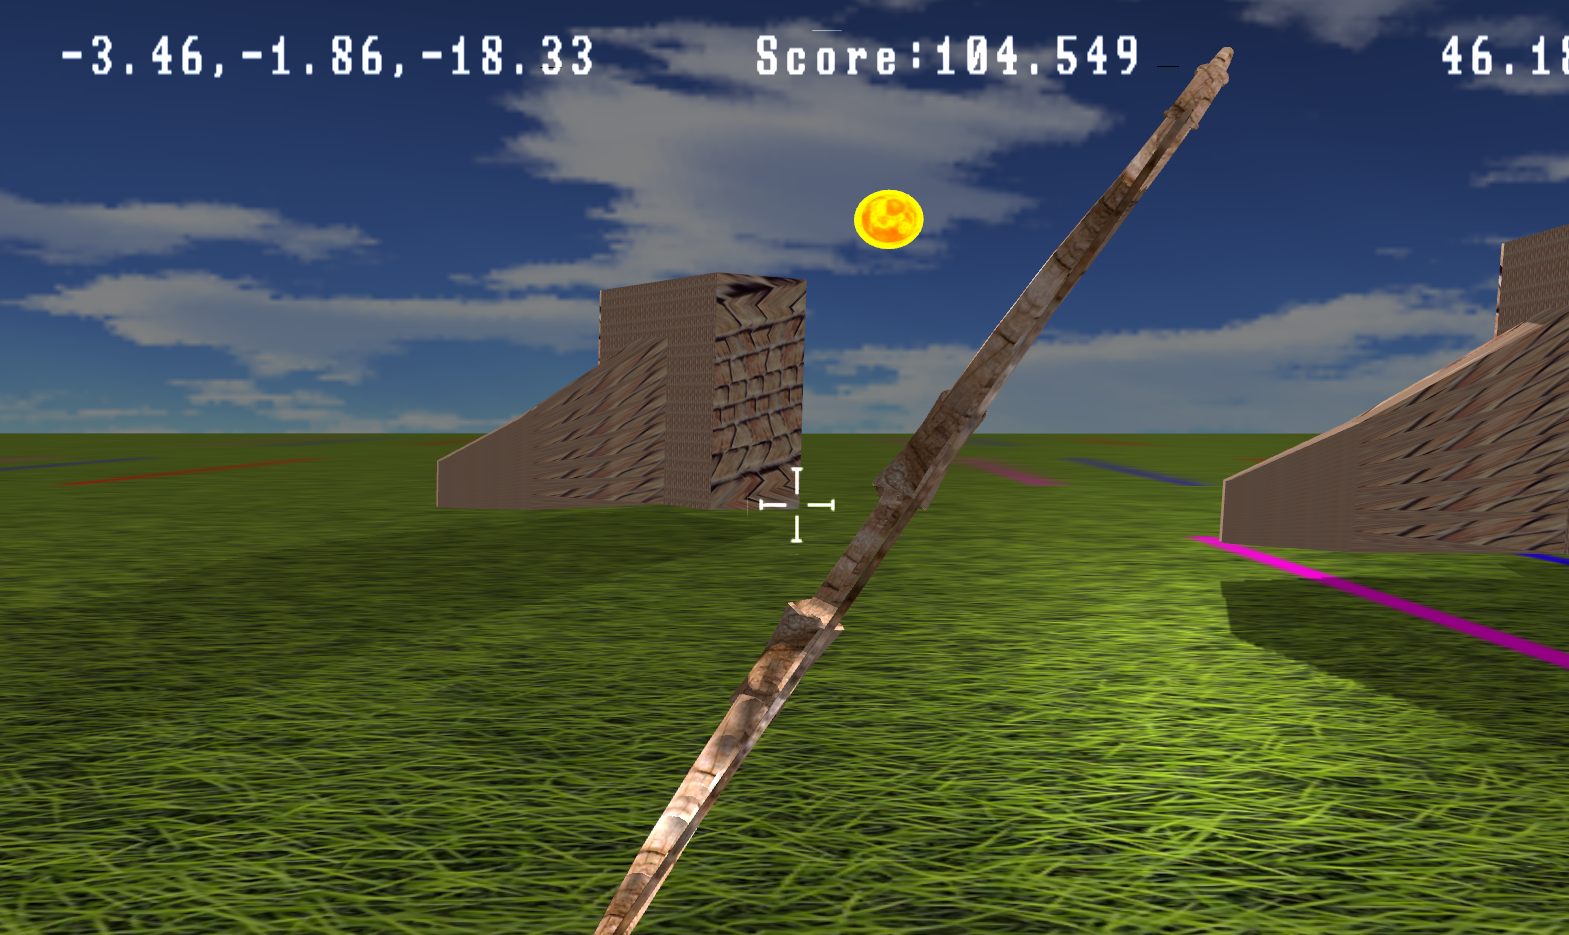
\includegraphics[scale=0.25]{obrazky-figures/23}
		\caption{Screenshot během úsvitu, jsou zde vidět stíny vržené terči a odlesk od vycházejícího slunce}\label{screenShot2}
\end{center}\end{figure}
\begin{figure}
	\begin{center}
			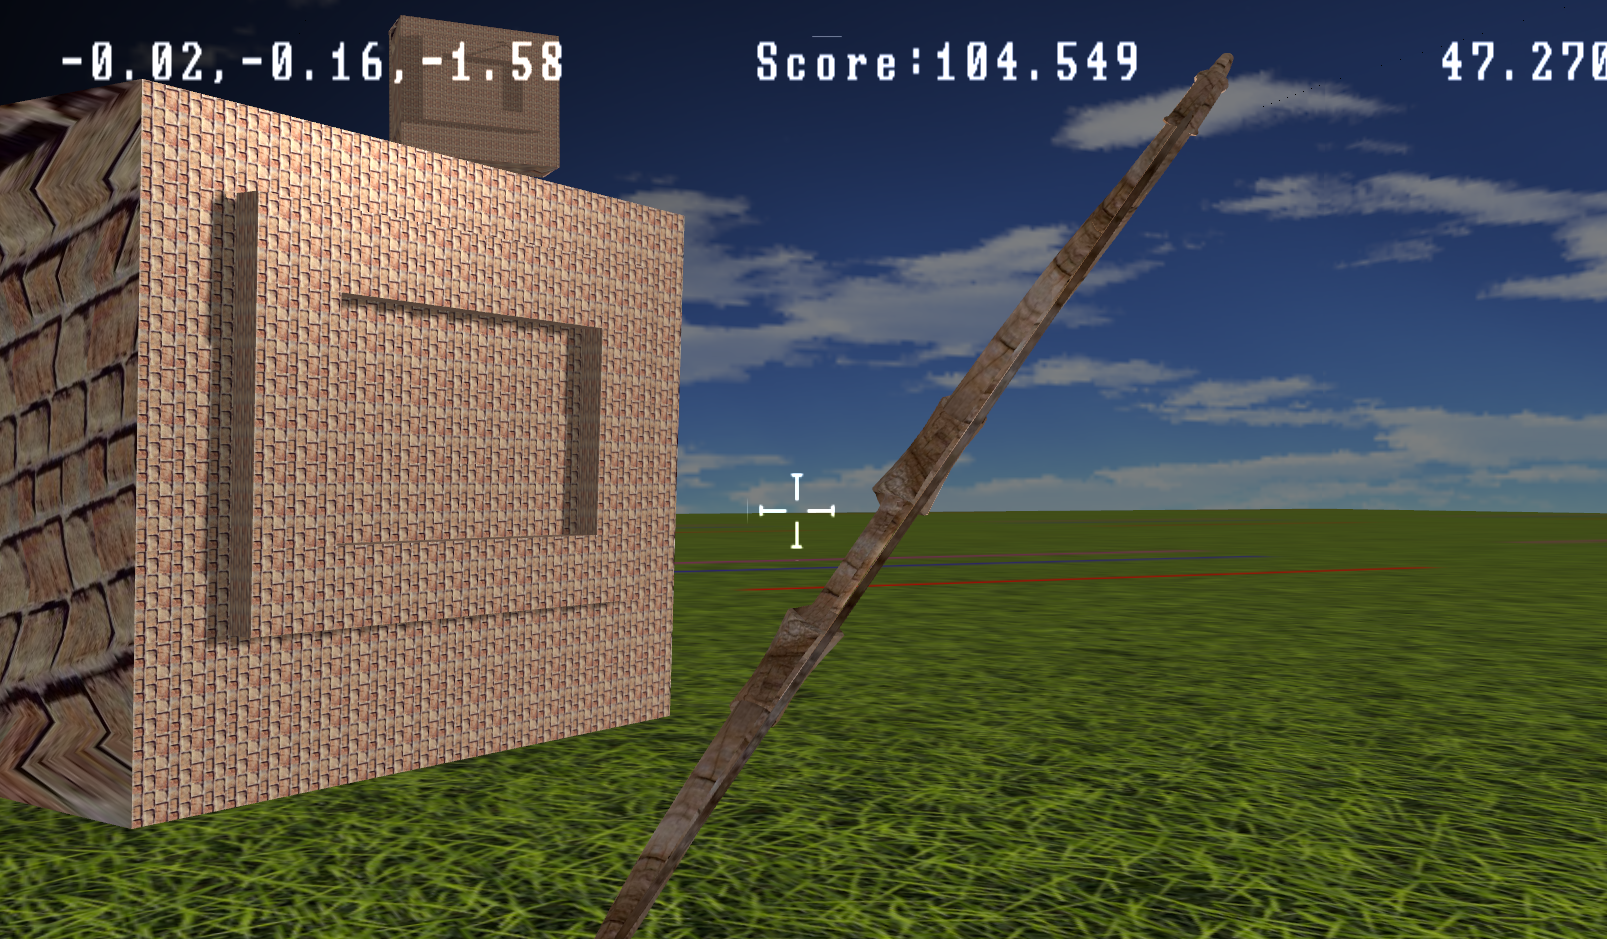
\includegraphics[scale=0.25]{obrazky-figures/24}
		\caption{Detail terče, na kterém jsou vidět vykreslené vlastní stíny}\label{screenShot3}
\end{center}\end{figure}

\begin{figure}
	\begin{center}
		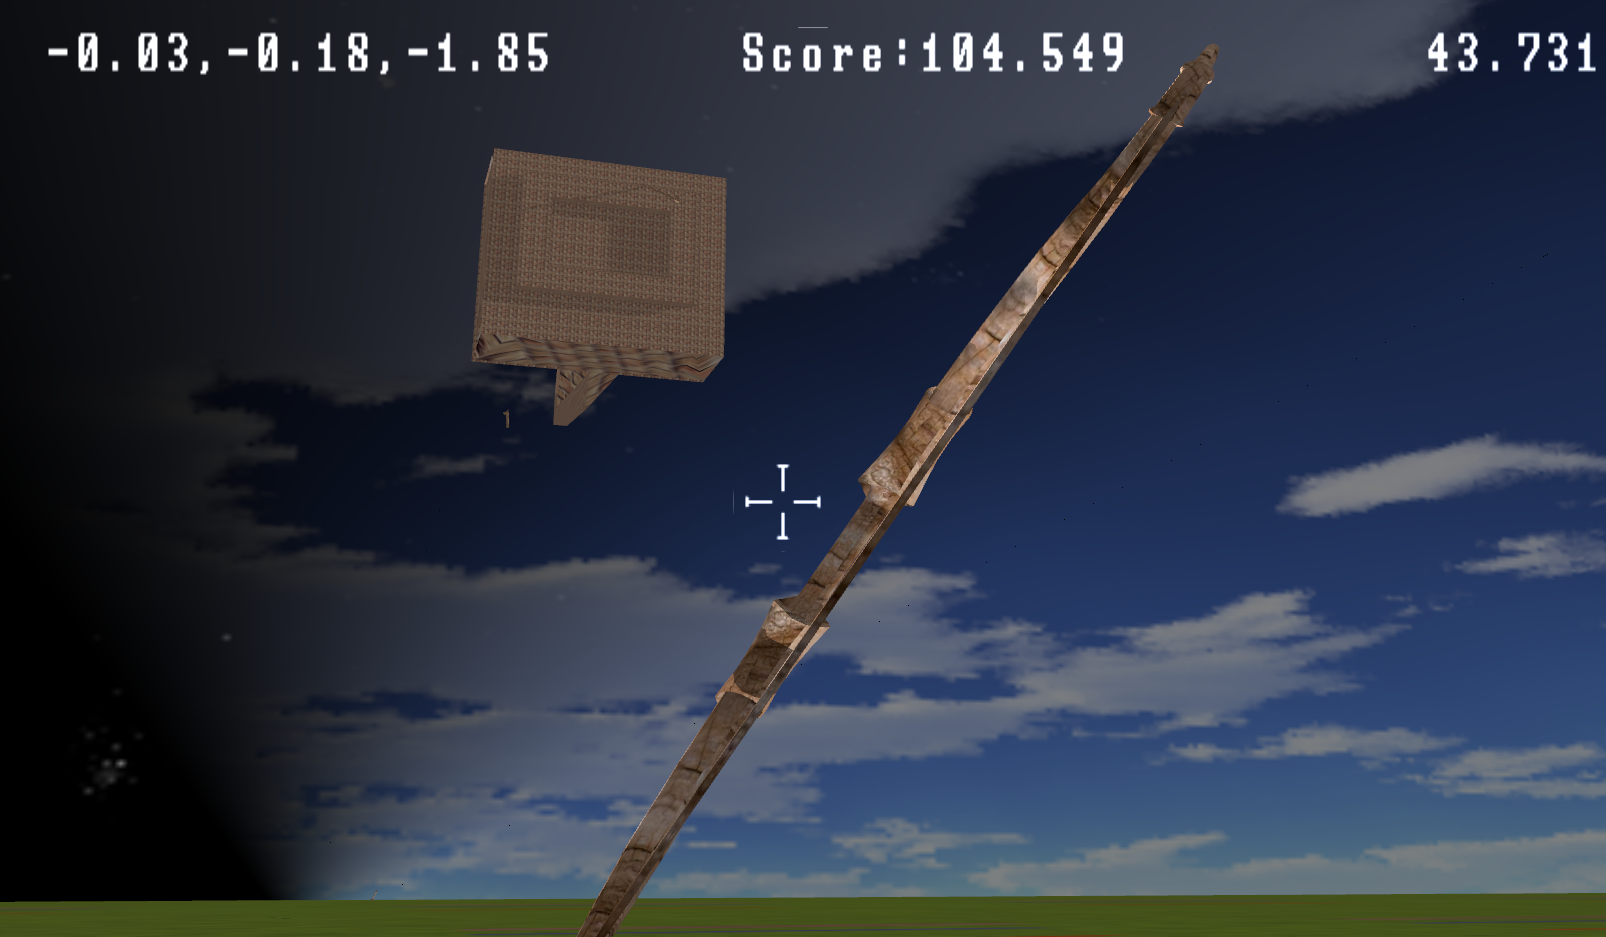
\includegraphics[scale=0.25]{obrazky-figures/27}
		\caption{Zde je vidět stín vržený zabodlým šípem v terči}\label{screenShot4}
\end{center}\end{figure}

\chapter{Obsah CD}
/ CD
\begin{itemize}
\item[/] \itab{3rd\_parties} 	\tab{-Obsah této složky je z převážné části tvorbou třetích stran} 					
	\begin{itemize}
	\item[/] \itab{authors.txt} \tab{-zde jsou uvedeny zdroje a autoři souborů v této složce.}
	\item[/] \itab{sounds} \tab{-složka obsahuje zvuky pro aplikaci}
	\item[/] \itab{libs} \tab{-externí knihovny}
	\item[/] \itab{icons} \tab{ -modely a textury}
\end{itemize}
\item[/] \itab{doc} \tab{ 			-zdrojové soubory technické zprávy}
\item[/] \itab{src} \tab{ 				-soubory aplikace}
	\begin{itemize}
		\item[/] \itab{InteractiveOpenGLDemo} \tab{ 	-zdrojové kódy výsledné aplikace a spouštěcí soubor pro 64-bit windows 10}
	\end{itemize}
\item[/] \itab{technická zpráva.pdf}
\end{itemize}